\newcommand{\PartidaMissao}{18h00}
\newcommand{\IbResposta}{Melhor combinação encontrada: velocidade \textbf{constante de \SI{20,5}{km/h}}, com partida às 18h00 (janela de 8\,h até 02h00); a viagem de \SI{7000}{km} termina em \textbf{214,8 dias} (\SI{32,6}{km/dia} em média) com reservas de 10\,\% na tração e 20\,\% nos serviços, ou 215,8 dias com reservas de 20/30\,\%.}
\newcommand{\IbResumo}{20,5 km/h constantes; 214,8 dias (31 km/dia em regime)}
\newcommand{\IbTexto}{%
A viagem parte com a tração cheia (\SI{98}{kWh} úteis) e o banco de serviços nominalmente cheio (\SI{14,4}{kWh} nominais) e só recebe energia solar. O tempo é contado a partir de 0h do primeiro dia, e a primeira partida é às 18h00: antes dela o veículo não roda, embora a janela diária de condução (18h00 a 02h00) cruze a meia-noite. A primeira chegada à reserva ocorre em 3,85 dias, após percorrer \SI{539}{km}; daí em diante cada dia roda o que o sol repôs, \SI{30,6}{km} em cerca de \SI{1,5}{h} de condução, bem abaixo do limite de 8\,h. Ao longo da viagem, os painéis geram \SI{3115}{kWh}: \SI{1300}{kWh} chegam à tração e \SI{1552}{kWh} abastecem a habitação (\SI{7,23}{kWh/dia}). A tração consome \SI{1383}{kWh} (\SI{0,198}{kWh/km}), em \SI{341}{h} de condução.

Como a energia solar diária é fixa, o tempo total é dominado pelos dias de espera para acumular energia, e não apenas pelas horas ao volante. O mínimo de consumo específico $v^{*}$ do item 27 é uma referência analítica para a busca; a agenda e as reservas ainda precisam ser verificadas. Nos casos comparados, rodar mais rápido aumenta o consumo e os dias de espera. Partir no fim da tarde deixa todo o período de sol com o veículo parado e os portáteis abertos. A Tabela~\ref{tab:i29comparacao} compara a melhor velocidade com 40 e \SI{80}{km/h} sob a mesma partida, as mesmas reservas e a mesma geração. A distância até a primeira vez que a tração atinge a reserva mede a autonomia com a bateria inicialmente cheia; o ritmo depois disso é o que a geração diária sustenta.
\IbComparacao

Em pista plana, o mínimo de consumo específico pode ser calculado diretamente (item 27), mas o tempo total também depende da agenda solar, da abertura dos portáteis, das reservas e da energia disponível em cada horário, interações que o simulador resolve intervalo a intervalo e que não têm forma fechada. Por isso a velocidade e o horário foram buscados numa grade; a velocidade publicada é a melhor combinação encontrada nas condições testadas, não um ótimo global demonstrado.

A melhor política foi localizada em duas etapas: varredura de \num{2784} combinações (\SIrange{12}{40}{km/h} a cada \SI{1}{km/h}, partida a cada \SI{0,5}{h}, duas reservas) com passo de \SI{5}{min}, e refino de \num{294} casos (passo de \SI{0,1}{km/h} e \SI{0,25}{h}) com passo de \SI{1}{min}; os líderes não estão na borda da grade local. Para o líder, entre passos de 5 e \SI{1}{min} a duração muda \SI{0,03}{dias}. A chegada é discretizada pela janela diária: se o último trecho não cabe antes do fim da janela, o veículo espera até a noite seguinte, de modo que uma pequena mudança de velocidade pode antecipar ou atrasar a chegada em quase um dia, como ocorre com as reservas de 20/30\,\%.

\textbf{Cenário opcional: acumular por mais de um dia.} Em vez de rodar todo dia o que o sol repôs, o veículo pode esperar alguns dias e percorrer um trecho maior depois, até 8\,h por dia. Essa política pode reduzir montagens, mas também altera o SOC, o espaço disponível nos bancos e o corte por capacidade; não se atribui a ela uma duração sem simulação específica. Devem ser mantidos o teto de 1560 Wp, o mínimo de 0,38 kW, as reservas e a ausência de energia da rede. A hipótese de dias claros repetidos, a recarga só pela interface CC e a operação diária dos portáteis continuam valendo; esse cenário não foi simulado.
\begin{figure}[H]\centering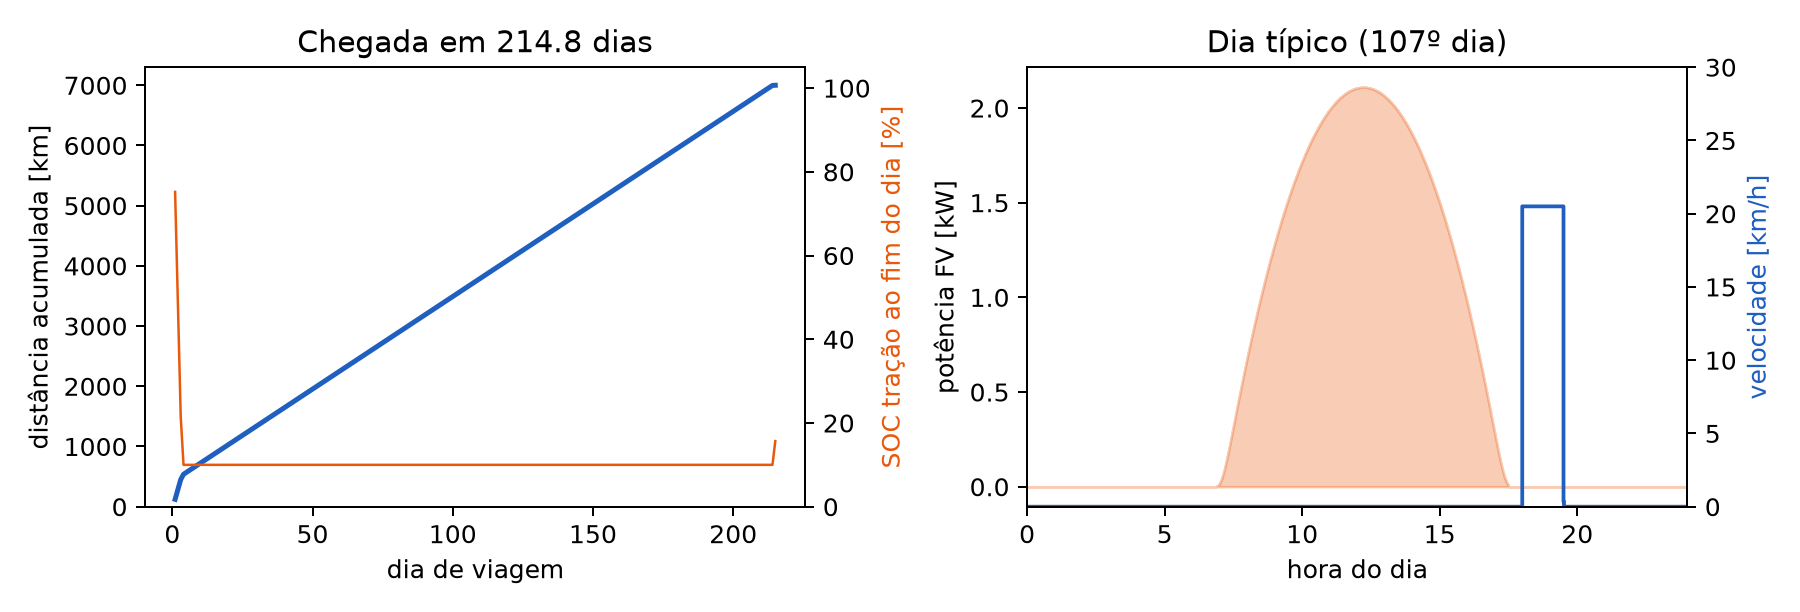
\includegraphics[width=\linewidth]{i29_missao.png}
\caption{Item 29 — distância acumulada e SOC da tração ao longo da viagem, e um dia típico.}\end{figure}}
\newcommand{\IbComparacao}{%
\begin{table}[H]\centering\small\setlength{\tabcolsep}{4pt}
\caption{Item 29 — mesma partida (18h00), mesmas reservas e mesma geração; só a velocidade muda.}
\label{tab:i29comparacao}
\begin{tabular}{rrrrrrr}
\toprule
$v$ & Viagem & Ao volante & Consumo & Até a reserva & \multicolumn{2}{c}{Depois da reserva} \\
{}[km/h] & [dias] & [h] & [kWh/km] & [km] & [km/dia] & [h/dia] \\
\midrule
20,5 & 214,8 & 341 & 0,198 & 539 & 30,6 & 1,49 \\
40,0 & 248,8 & 175 & 0,228 & 414 & 26,7 & 0,67 \\
80,0 & 457,8 & 88 & 0,408 & 216 & 14,8 & 0,19 \\
\bottomrule
\end{tabular}
\end{table}}
